\documentclass[10pt, a4paper]{article} % 设置字体大小和纸张类型
\usepackage{booktabs} % 支持更专业的表格线条
\usepackage{ctex}
\usepackage{caption} % 插图和表格的标题格式
\usepackage{amsmath, amsfonts, amssymb} % 数学公式支持
\usepackage{graphicx} % 插入图片
\usepackage{hyperref} % 超链接支持
\usepackage{geometry}
\usepackage{titlesec}
\usepackage{fmtcount} % 用于数字到中文的转换
\usepackage{enumitem} % 加载 enumitem 宏包
\usepackage{multirow} % 支持多行单元格
\usepackage{diagbox}
\geometry{a4paper, margin=1.5cm} % 设置页边距

\renewcommand{\thesection}{\chinese{section}、}
\renewcommand{\thesubsection}{\arabic{subsection}.}


\begin{document}

\begin{titlepage}
    \newgeometry{left=0cm, right=0cm, top=0cm, bottom=0cm}
    \centering
    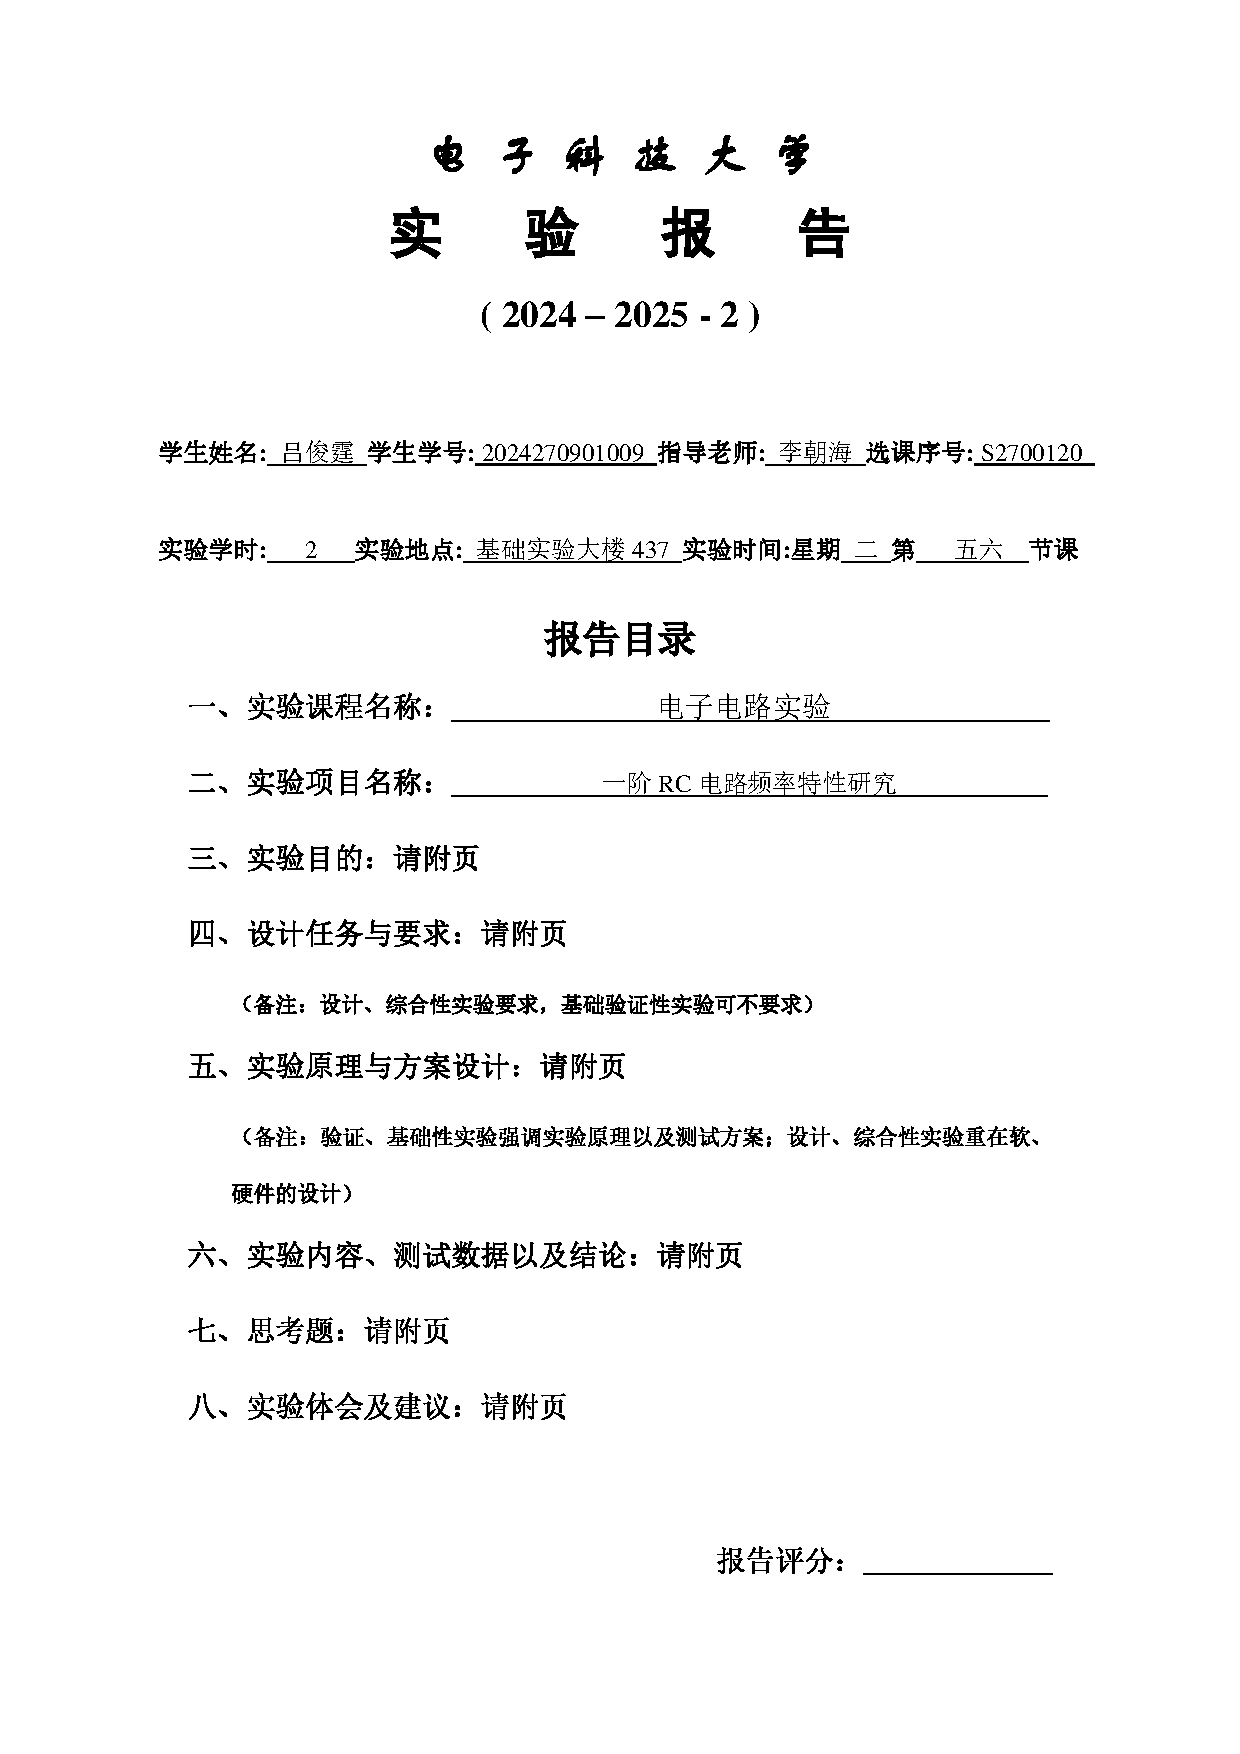
\includegraphics[page=1, width=0.9\textwidth, keepaspectratio]{image/实验报告撰写封面.pdf}
    \restoregeometry
\end{titlepage}

\setcounter{section}{2}

\section{实验目的}

\begin{enumerate}[leftmargin=50pt,label=(\arabic*)] % 设置序号格式为(1)
    \item 了解动态电路的正弦稳态响应以及求解方法; 
    \item 了解网络频率响应的基本概念; 
    \item 掌握网络频率特性测试的一般方法; 
    \item 研究一阶RC电路的幅频特性和相频特性。
\end{enumerate}

\section{设计任务与要求}

\begin{enumerate}[leftmargin=50pt,label=(\arabic*)] % 设置序号格式为(1)
    \item 预习正弦稳态响应的阻抗模型求解方法;
    \item 根据直觉画出RC和RL电路的频率响应示意图;
    \item 预习滤波器基本概念以及分类;
    \item 预习滤波电路的通频带和电路参数之间的关系;
    \item 试用RC器件设计一阶低通滤波器, 并计算出其截止频率;
\end{enumerate}

\section{实验原理与方案设计}
\subsection{实验原理}
工程中常用频率响应(也就是正弦响应)来表征系统的特性。求解电路的正弦稳态响
应通常可用阻抗分析法, 即: 将正弦激励用其复幅值替代, 电阻用R替代, 电容用1/sC
(或1/j$\omega$ C)替代, 电感用sL(或j$\omega$L)替代,则可求出任意线性RLC网络的电压电流复
幅值之间的关系,复幅值同时携带了响应的幅值和相位的信息。

传递函数,也称为系统函数,是网络输出复幅值与输人复幅值的比值。频率响应是指
网络传递函数的幅值和相位作为频率的函数图形,分别称为幅频响应和相频响应。电路的
频率响应表明了它们的频率选择性,可以依据这种电路来处理信号,这样使用的电路就称
为滤波器。滤波器是频域分析的一类重要应用,根据电路对频率的选择性,滤波器通常可
以分为低通滤波器、高通滤波器、带通滤波器以及带阻滤波器等几种类型。


一阶RC低通滤波器


如图1是一阶RC串联低通滤波器, 若一电容两端的电压作为输出, 该电路具有低通的滤波特性。该电路的网络传递函数为
$$
H(j\omega) = \frac{V_{out}(j\omega)}{V_{in}(j\omega)} = \frac{1}{1 + j\omega RC}
$$
$$
=\frac{1}{\sqrt{1 + (\omega RC)^2}} \cdot \angle - \arctan(\omega RC)
$$
$$
=\left\lvert H(j\omega)\right\rvert \cdot \angle \theta (\omega)
$$

可以看出, H(j$\omega$)除了和电路结构及元件参数有关以外, 还是频率$\omega$的函数。其中, $\left\lvert H(j\omega)\right\rvert$是幅频特性, $\theta(\omega) = -\arctan(\omega RC)$是相频特性。令$\omega_0= \frac{1}{RC}$, 成为网络的固有频率,则有
$$
\left\lvert H(j\omega_c)\right\rvert = \frac{1}{\sqrt{1+(\frac{\omega}{\omega_0})^2}}
$$
$$
\theta(\omega_c) = -\arctan\frac{\omega}{\omega_0}
$$

电路的幅频特性和相频特性统称为电路的频率特性。将传递函数的模随频率变化的曲线称为幅频特性曲线, 将传递函数的相角随频率变化的曲线称为相频特性曲线。一阶RC低通滤波器的幅频特性如图2所示, 相频特性曲线如图3所示。

\newpage

\begin{figure}[ht]
    \centering
    \begin{minipage}[ht]{0.3\textwidth}
        \centering
        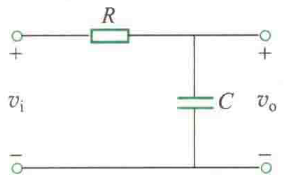
\includegraphics[width=\linewidth]{image/1.png}
        \caption{一阶RC串联低通滤波器}
        \label{fig:side:a}
    \end{minipage}
    \hfill
    \begin{minipage}[ht]{0.3\textwidth}
        \centering
        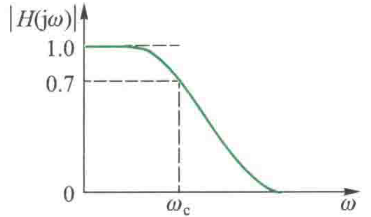
\includegraphics[width=\linewidth]{image/2.png}
        \caption{幅频特性曲线}
        \label{fig:side:b}
    \end{minipage}
    \hfill
    \begin{minipage}[ht]{0.3\textwidth}
        \centering
        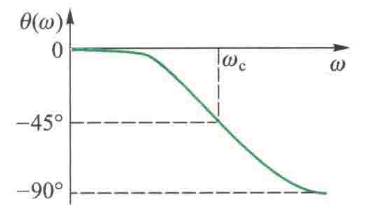
\includegraphics[width=\linewidth]{image/3.png}
        \caption{相频特性曲线}
        \label{fig:side:c}
    \end{minipage}
\end{figure}

对于滤波器, 工程上一种常用的定义是当功率正好下降到最大输出功率的1/2时, 即输出电压的幅度刚好衰减到通带输出幅度的0.707时, 所对应的频率为截止频率, 记为$\omega_c$。 容易看出该RC滤波电路中$\omega_c = \omega_0$。


\subsection{方案设计}
使用点频法测量幅频特性曲线, 即在输入信号电压值保持不变的情况下, 改变输入信号的频率, 测量输出信号的幅度, 从而得到幅频特性曲线。

截止频率的测试可以按照以下步骤进行:

第一步:将函数发生器接人待测网络的输人端并提供正弦信号,设定输人电压大小
(用交流毫伏表测试,并保持后续测试中该电压值恒定);

第二步:寻找该网络在上述输人电压条件下的通带输出电压。调节函数发生器的频
率,用交流毫伏表观察输出电压变化情况,记录该网络能达到的(平坦区)最大输出电
压值。

第三步: 测试截止频率。根据定义, 第二步测到的电压值的0.707所对应的输入信号
频率即为截止频率。调节函数信号发生器的频率,用交流毫伏表观察输出电压值,当输出
电压达到通带输出电压值的0.707时,记录函数发生器的频率读数,即为截止频率。需要
注意的是,读数时要保证输人电压不变。

\section{实验内容、测试数据以及结论}
一阶RC低通滤波器的测量

\begin{table}[htbp]
    \centering
    \caption{一阶 RC 低通滤波器的频率特性测试数据}
    \label{tab:rc_filter_data}
    \begin{tabular}{|c|c|c|c|c|c|c|c|}
    \hline
    \multirow{2}{*}{输入信号频率 $f/\text{Hz}$} & \textbf{$0.01f_c$} & \textbf{$0.1f_c$} & \textbf{$0.5f_c$} & \textbf{$f_c$} & \textbf{$2f_c$} & \textbf{$5f_c$} & \textbf{$10f_c$} \\ \cline{2-8}
    &149  &1.49K  &7.49K  &14.98K  &29.96K  &74.96K  &149.8K  \\ \hline % 仅合并第一列,其他列不受影响
    输出信号 $V_o/\text{V}$ &1.05  &1.00 &0.88 &0.7 &0.45 &0.2 &0.1 \\ \hline
    输出与输入信号相位差 $\theta/^\circ$ &\diagbox{}{} &\diagbox{}{} &\diagbox{}{} &$45^{\circ}$ &\diagbox{}{} &\diagbox{}{} & \diagbox{}{}\\ \hline
    \end{tabular}
\end{table}

\begin{figure}[ht]
    \centering
    \begin{minipage}[ht]{0.56\textwidth}
        右图为用MATLAB绘制的曲线
    \end{minipage}
    \hfill
    \begin{minipage}[ht]{0.4\textwidth}
        \centering
        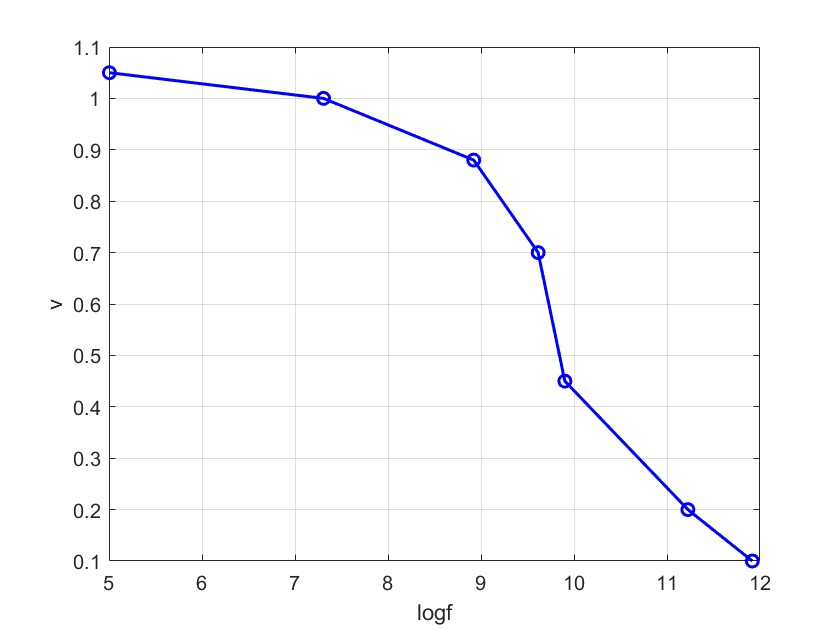
\includegraphics[width=\linewidth]{image/1.jpg}
        \caption{MATLAB绘图结果}
        \label{fig:side:ii}
    \end{minipage}
\end{figure}

\newpage

\section{思考题}
\subsection{题面}
\begin{enumerate}[leftmargin=50pt,label=(\arabic*)] % 设置序号格式为(1)
    \item 在测量幅频特性曲线时, 为什么强调要保持输入信号的大小保持不变?
    \item 函数发生器接人含动态元件的待测网络输人端口时,改变函数发生器的频率(没有调节输出幅度旋钮),待测网络的输入电压有可能发生了变化,为什么?
    \item 在测相位差时,为什么要尽可能保证示波器两个通道的零基线与荧光屏的横坐标重合?
    \item 信号源有50Ω的内阻, 在选取RC元件参数时, 为什么应尽量避免选取小电阻?
\end{enumerate}
\subsection{回答}

\begin{enumerate}[leftmargin=50pt,label=(\arabic*)] % 设置序号格式为(1)
    \item 输出大小与输入频率和大小有关, 不包吃大小不表不符合单一变量原则
    \item 输入阻抗是一个复数, 与频率和相位有关, 阻抗会发生变化, 影响待测网络输入电压
    \item 因为这时候相位差准确
    \item 小电阻会导致电压波动太大, 影响实验结果
\end{enumerate}

\section{实验体会及建议}
\subsection{实验体会}
通过本次实验, 我更好地理解了一阶RC电路的基本特性, 可以熟练使用函数发生器, 毫伏表和示波器
\subsection{建议}
误差较大, 应该多次测量比例减小误差


\end{document}
